Reinforcement learning is the process of learning what to do to maximize a numerical reward. A mechanism where the learner is not told what action to take, but instead must discover which action yields the highest reward by trying them. In this case, actions might affect not only the immediate reward but also future situations and all the subsequent rewards. These two characteristics -- Trial-and-error search and delayed reward -- are the two most important distinguishing features of reinforcement learning.

Reinforcement learning differs from supervised learning since training is not based on an external dataset of labeled examples, where each situation (observation) is labeled with the correct action to perform (often identify a category). RL, although one might erroneously think the opposite, is also different from unsupervised learning. The main objective for unsupervised learning is to find hidden structures in an unlabeled dataset, whereas RL's main objective is to maximize a reward signal. 

In this chapter, we will see the definition of a Markov decision process and those of the state and action value function. Afterward, we will observe how optimization is carried out in an approximate solution method, in particular in the case of the proximal policy optimization since it is the technique utilized for training the neural network.

\section{Finite Markov Decision process (MDPs)}

Finite Markov decision processes are a class of problems that formalize subsequent decision making, where not only the influence of the action is exerted on immediate reward but also on those in the future. MDP's are suited for RL since they frame the process of learning through repeated interaction between an agent (decision maker), and an environment (ruled by fixed state transition function).

More specifically an agent is asked to take an action \( a_t \in \mathcal{A} \) at every time step \( t = 0,1,...\, \). To do so the agent is provided with an observation of the current environment's state \( s_t \in \mathcal{S} \) and a reward \( r_t \in R \) from the previously performed action. Afterwards the environment update it
s state following a transition distribution \( \mathcal{T}(s_{t+1}|a_t,s_t) \) and a numerical reward \( r_{t+1} \in \mathcal{R} \subset \mathbb{R} \). This process is reproduced every subsequent timestep, this concatenation of interaction is a MDP.

\begin{figure}[!h]
  \centering
  \linespread{.9}
  \begin{tikzpicture}[node distance=1cm, auto,]
      \node[punkt] (agent) {Agent};
      \node[punkt, inner sep=5pt,below=1cm of agent] (env) {Environment};
      \path[draw,->] 
        (env.west) -- ++(0cm,.1cm)  -- ++(-1cm,0cm) -- ++(0,1.65cm)  -- ++(1cm,0cm);
      \path[draw,->] 
        (env.west) -- ++(0cm,-.1cm) -- ++(-1.6cm,0cm) -- ++(0,2.05cm) -- ++(1.6cm,0cm);

      \path[draw,->] 
        (agent.east) -- ++(1.25cm,0cm) -- ++(0,-1.85cm) -- (env.east);


      \draw (3.1,-1) node[] {\( a_{t} \)};
      \draw (-2,-1) node[] {\( r_{t+1} \)};
      \draw (-3.5,-1) node[] {\( s_{t+1} \)};
  \end{tikzpicture}
  \caption[Agent enviroment interaction dynamic: ]%
  {\label{img:a-e_dynamic}Agent enviroment interaction dynamic: \small \textit{this is the basic dynamic of the interaction between the agent and the enviroment in a MDP, at time t the agent provides an action a and the enviroment respond with a state s and rewad r that are used from the agent to decide the action at t+1 and so on.}}
\end{figure}


\paragraph{Objective and Rewads:} The main objective of RL is to maximize the total number of rewars it receive. This reward \( r_t \) is passed from the environment to the agent at every timestep as a consequence of his actions. In the case of the Gather and Trade the reward is \( r_{i,t} = u_i(x_{i,t},l_{i,t})  - u_i(x_{i,t-1},l_{i,t-1}) \). 

Since the agents want to maximize the total upcoming reward we can write this value simply as the sum of all the future rewards.

\begin{equation*}
U_t \doteq r_{t+1} + r_{t+2} + ... + r_{H},
\end{equation*}

Where \( H \) is the total length of the episode, and at the time step \( t = H \) the episode ends. This state is called the terminal state and is a particular state because regardless of the final condition of the agent it reset the environment to the initial condition and restart completely the episode.
Another specification for the total reward can implement the concept of discounting, which is more appropriate in the case of economical simulations, thus within the experiments the agent has to maximize his future discounted utility:

\begin{equation}
U_t \doteq r_{t+1} + \gamma r_{t+2} + \gamma^2 r_{t+3} +... + \gamma^{H-t-1}r_{H},
\end{equation}

the discount rate \( \gamma \in [0,1] \) determines the value that the agent assigns to the future reward, a reward received at \( k \) timesteps in the future is only valued \(\gamma^{k-1} \) times what it would be valued today. When the value of \( \gamma \) approaches 0 the agent is more "myopic" and puts most of his interest in immediate rewards, while if it approaches 1 the interest is more projected in the future due to the stronger impact of future rewards.

\paragraph{Value functions: } One of the most important elements of RL is the value function. The estimation of this function is one of the crucial points of RL, in fact it tries to quantify the expected return of the rewards it expects to receive. Furthermore, the expected reward depends on the action that the agent decides to take, thus the value function are defined in terms of policies, which are acting behaviors.

If the agent is following policy \( \pi \) at time \( t \), then \( \pi(a|s) \) is the probability that the agent takes the action \( a_t = a \) given the state \( s_t = s \). The aim of RL is to change the policy based on experience across episodes to find an optimal behavior.

We can write a value funciton for a state \( s \) under the policy \( \pi \). This function is the expected return when the inital state is \( s \) and the policy followed is \( \pi \).

\begin{equation}
v_\pi(s) \doteq \mathbb{E} _\pi \left[ U_t | s_t = s \right] \, =\,  \mathbb{E} _\pi \left[\left.\sum_{k = 0}^{H}\gamma^k r_{t+k+1}  \right| s_t = s \right], \quad \text{for all}\, s \in \mathcal{S} 
\label{eq:statevalue_function}
\end{equation}

\(  v_\pi(s)\) is called the state-value function for policy \( \pi \). Following from this equation, it is possible to define the value of taking an action \( a \) in the state \( s \) following the policy \( \pi \):

\begin{equation}
    q_\pi(s,a) \doteq \mathbb{E} _\pi \left[ U_t | s_t = s, a_t = a \right] \, =\,  \mathbb{E} _\pi \left[\left.\sum_{k = 0}^{H}\gamma^k r_{t+k+1}  \right| s_t = s, a_t = a \right],
    \label{eq:actionvalue_function}
\end{equation}
    
and \( q_\pi(s,a) \) is called the action-value function for policy \( \pi \). The important concept here is that the value functions in \ref{eq:statevalue_function} and \ref{eq:actionvalue_function} can be estimated from experience. 

There are multiple strategies to determine an optimal behavior starting from the evaluation of these functions, we can divide these ways in two main groups, tabular solution methods and approximate solution methods\cite{sutton2018reinforcement}. For the former we have Montecarlo methods, Dynamic programming, Temporal-difference learing, n-step bootsrap and others. While for the latter we have On/Off-policy methods with approximation and policy gradient methods. 

For the purpose of this thesis we are going to foucs only on policy gradient methods and a particular set of optimization policy called proximal policy optimization.

\section{Approximate solution Methods}

The approximate solution methods are sets of strategies thought for those problems, such as ours, where the set of possible states is enormous. It is very likely that every state encountered in a simulation will never have been encountered before. Thus, to make meaningful decisions there is the need to be able to generalize from previous state that are, to some extent, similar. This is accomplished by borrowing the exising generalization theory, usually by using the process of function aproximation. However, we are going to use policy gradient methods that do not necessarily need to estimate a value function through function aproximation. 



\subsection{Policy gradient Methods}  


Policy gradient methods are a set of parameterized policies that can select actions without the use of a value function. The method consists in calculating the estimator of the policy gradient and feeding it into a stochastic gradient ascent algorithm. We denote with \( \pi_\theta(a|s) \) the stochastic policy such that 
\begin{equation}
  \pi_\theta(a|s) = \pi(a| s, \mathbf{\theta}) = Pr \left\{ a_t = a | s_t = s \, , \,   \mathbf{\theta}_t =  \mathbf{\theta}\right\}
\end{equation}
for the probability of choosing action \( a \) at time \(  t \) given the state \( s_t \) and the parameters \(  \mathbf{\theta} \). The aim of the policy gradient methods is to maximize a perfomance measure \( J_t( \mathbf{\theta}) \). This is done by updating the parameters \(  \mathbf{\theta} \) with a gradient of the performance itself:

\begin{equation}
  \mathbf{\theta}_{t+1} =  \mathbf{\theta}_t + \alpha\widehat{\nabla J ( \mathbf{\theta}_t)}
\end{equation}



\subsection{Proximal Policy Optimization Algorithms}

Proximal policy optimization algorithms (PPOs) are a family of policy gradient methods for reinforcement learning, which alternate between sampling data through interaction with the environment, and optimizing a "surrogate" objective function using stochastic gradient ascent. 

PPO utilizes as a performance measure the advantage \( A(s,a) = q(s,a) - v(s) \), which represents how good an action is compared to the average action in a specific state.

It also relies on the ratio of the policy that we want to refine to the older policy:

\begin{equation}
r_t(\theta)= \frac{\pi_\theta(a_t|s_t)}{\pi_{\theta old}(a_t|s_t)}
\end{equation}

The surrogate objective function that we optimize with PPO is 

\begin{equation}
\mathcal{L}^{CLIP} (\theta) = \hat E_t \left[ min(r_t(\theta)\hat A_t \,, \, clip(r_t(\theta) \,,\, 1-\epsilon\,,\, 1+ \epsilon)\hat A_t)\right]
\end{equation}

The maximization of this surrogate funcition takes the advantages of trust region policy optimization (TRPO) \cite{schulman2015high}, adjusting the parameters in the dierction of the ratio \( r_t(\theta) \), and maintaining this change bounded in a "clipped" region to avoid drastic refinements of the policy. This is shown well in the Figure \ref{img:l_clip}


\begin{figure}[h!]
  \centering
  \linespread{.9} 
  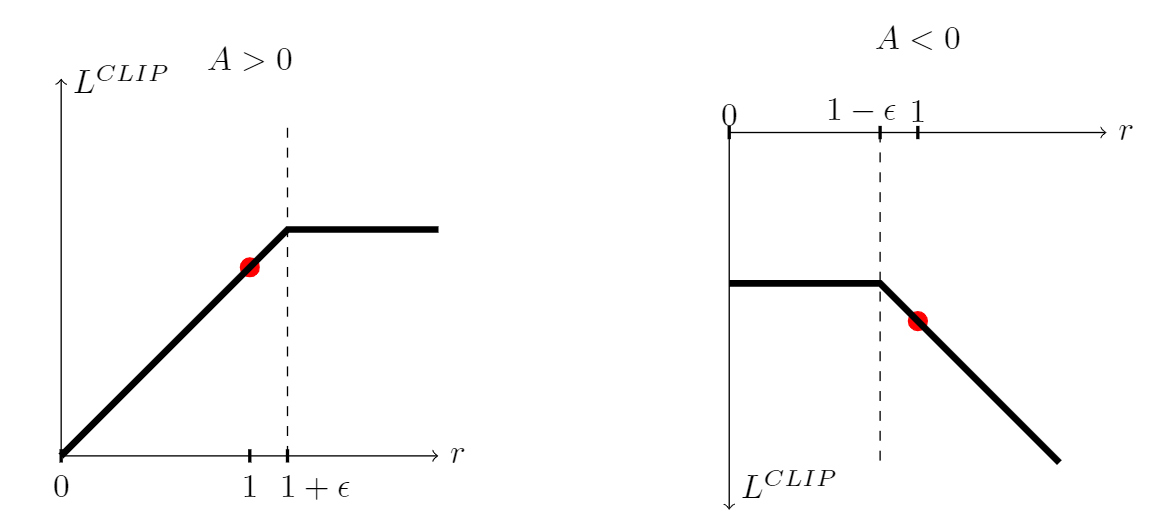
\includegraphics[width=0.75\textwidth]{Resources/imgs/L_clip.PNG}
  \caption[One step \( L^{CLIP} \) as a function of \( r_t(\theta) \):  ]%
  {\label{img:l_clip}One step \( L^{CLIP} \) as a function of \( r_t(\theta) \): \small \textit{this is the function \( L^{CLIP} \) as a function of the probability ratio \( r_t(\theta) \) when the advantage A is positive or negative. The red dot is the starting point of the optimization. (Figure from \cite{schulman2017proximal})}}
\end{figure}


The surrogate function can be further augmented by adding an entropy bonus to ensure sufficient exploration. By adding these terms, we obtain the following objective function:

\begin{equation}
L_t^{CLIP+VF+S}(\theta) = \hat E_t \left[ L_t^{CLIP}(\theta) - c_1 L_t^{VF}(\theta)  + c_2 S[\pi_\theta](s_t)\right]
\end{equation}

where \( S \) in an entropy bonus, \(  L_t^{VF} \) is a squared-error loss and \(c_1, c_2 \) are coefficients.

The pseudocode below better explains all the procedure done by the PPO in refining the parameters.

\begin{algorithm}
  \caption{PPO with clipped objective}\label{alg:ppo_clip}
  \begin{algorithmic}
    \State Input: inital policy \( \theta_0 \), clipping threshold \( \epsilon \)
    \For{\( k = 0,1,2... \)}
      \State Collect a set of trajectories $\mathcal{D}_k$ on policy \( \pi_k = \pi(\theta_k) \)
      \State Estimate the adventages \( \hat A_t^{\pi_k} \), using any advantage est. alg. 
      
      \Comment{we will use GAE\cite{schulman2015high}}
      \State Compute policy update
      \begin{equation*}
        \mathbf{\theta}_{k+1} = arg \max_\theta \mathcal{L}^{CLIP}_{\theta_k}(\theta)
      \end{equation*}
      \State by taking K steps of minibatch SGD (via Adam \cite{kingma2014adam}), where
      \begin{equation*}
        \mathcal{L}^{CLIP}_{\theta_k}(\theta) =  E_t \left[ \sum_{t=0}^T\left[  min(r_t(\theta)\hat A^{\pi_k}_t \,, \, clip(r_t(\theta) \,,\, 1-\epsilon\,,\, 1+ \epsilon)\hat A_t^{\pi_k})\right]\right]
      \end{equation*}
    \EndFor
  \end{algorithmic}
\end{algorithm}



\begin{comment}

One of the most often used gradient estimator uses the following formula:

\begin{equation}
\hat g = \hat E_t \left[ \nabla_\theta log \pi_\theta ( a_t | s_t) \hat J_t  \right]
\end{equation}

Here the expected value is taken over a minibatch in an algorithm that alternates sampling and optimization.

  \bigskip


\begin{algorithm}
  \caption{basic PPO structure}\label{alg:cap}
  \begin{algorithmic}
      \For{iteration = 1,2 ...}
      \For{actor = 1,2,..., N}
        \State Run policy \( \pi_{\theta_{old}} \) in enviroment for \( T \) time-steps
        \State Compute advantage estimate \( \hat A_1 , ... , \hat A_T \)
      \EndFor
      \State Opt. surrogate \( L \) wrt \( \theta \), with K epochs and minibatch size \( M \leq NT \)
      \State $\theta_{old} \gets \theta$
    \EndFor
  \end{algorithmic}
\end{algorithm}

\end{comment}




